\documentclass{article}

\usepackage{fullpage}
\usepackage{graphicx}
\usepackage{color}
\usepackage{fancyhdr}
\usepackage{url}
\usepackage{amsmath,bm}
\usepackage{amssymb}
\usepackage{amsthm}
\usepackage{amsfonts}
\usepackage[round]{natbib}
\usepackage{enumitem,xcolor}
\usepackage[multiple]{footmisc}

\graphicspath{ {figures/} }

\usepackage[
    pdftitle={Capstone Proposal - Udacity Machine Learning Nanodegree},
    pdfsubject={Machine Learning, Reinforcement Learning, Deep Learning, Artificial Intelligence, Games},
    pdfauthor={David Robles},
    pdfpagemode=UseOutlines,
    pdfborder= {0 0 1.0},
    bookmarks,
    bookmarksopen,
    colorlinks=true,
    citecolor=blue,
    linkcolor=blue, %
    linkbordercolor=blue, %
    urlcolor=blue, %
]{hyperref}

\usepackage[labelfont=bf]{caption}


\usepackage[utf8]{inputenc}

% Default fixed font does not support bold face
\DeclareFixedFont{\ttb}{T1}{txtt}{bx}{n}{8} % for bold
\DeclareFixedFont{\ttm}{T1}{txtt}{m}{n}{8}  % for normal

% Custom colors
\usepackage{color}
\definecolor{deepblue}{rgb}{0,0,0.5}
\definecolor{deepred}{rgb}{0.6,0,0}
\definecolor{deepgreen}{rgb}{0,0.5,0}

\usepackage{listings}

\definecolor{codebg}{RGB}{238,238,238}

% Python style for highlighting
\newcommand\pythonstyle{\lstset{
language=Python,
basicstyle=\ttm,
otherkeywords={self},             % Add keywords here
keywordstyle=\ttb\color{deepblue},
emph={MyClass,__init__},          % Custom highlighting
emphstyle=\ttb\color{deepred},    % Custom highlighting style
stringstyle=\color{deepgreen},
frame=tb,                         % Any extra options here
framesep=10pt,
framexleftmargin=10pt,
backgroundcolor=\color{codebg},
rulecolor=\color{codebg},
aboveskip=15pt,
belowskip=15pt,
showstringspaces=false            %
}}


% Python environment
\lstnewenvironment{python}[1][]
{
\pythonstyle
\lstset{#1}
}
{}

% Python for external files
\newcommand\pythonexternal[2][]{{
\pythonstyle
\lstinputlisting[#1]{#2}}}

% Python for inline
\newcommand\pythoninline[1]{{\pythonstyle\lstinline!#1!}}



%%%%%%%%%%%%%%%%%%%%%%%%%%%%%%%%%%%%%%%%%%%%%%%%%%%%%%%%%%%%%%%%%%%%%%%%%%%%%%%%%%%%%%%%%%%%%%%%%%%%
\title{Machine Learning Nanodegree \\ Capstone Proposal}
\author{Sam Mottahedi}
\date{01/08/2018}
\begin{document}
\maketitle


\section{Definition}

    \subsection{Project Overview}

    Natural language processing (NLP) is one of the most important technologies of the information age. Understanding complex language utterances is also a crucial part of artificial intelligence. Applications of NLP are everywhere because people communicate most everything in language: web search, advertisement, emails, customer service, language translation, radiology reports, etc. There are a large variety of underlying tasks and machine learning models behind NLP applications.


    \subsection{Problem Statement}


    Free expression and sharing information is the greatest impact of internet in modern society. Unfortunately, online abuse and harassment can lead limit self expression on the web. Many platforms struggle to effectively
    facilitate conversations, leading many communities to limit or
    completely shut down user comments.


    In this \href{https://www.kaggle.com/c/jigsaw-toxic-comment-classification-challenge}{Kaggle competition} ,  participant are challenged to build a multi-headed model that’s capable of detecting different types of of toxicity like threats, obscenity,insults, and identity-based hate.


    \subsection{Metrics}

    Submissions are evaluated on the mean column-wise log loss. In other words, the score is the average of the log loss of each predicted column.


    Since class labels are not mutually exclusive, a multi-label classification loss function is required here. Multi-label classification (MLC) is a prediction problem in which several class labels are assigned to single instances simultaneously as follows:

    \begin{equation}
            loss(\hat{y}, y) = \frac{1}{|L|} \sum_{l=1}^{l=|L|} - (y_l - log(\hat{y_l}) + (1-y_l) \cdot log(1-\hat{y_l}))
    \end{equation}



\section{Analysis}

    \subsection{Data Exploration}

    The \href{https://www.kaggle.com/c/jigsaw-toxic-comment-classification-challenge/data}{Kaggle competition dataset} provided is Wikipedia Human Annotations of Toxicity on Talk Pages and contains $160,000$ human labelled annotations based on asking 5000 crowd-workers to rate Wikipedia comments according to their toxicity (likely to make others leave the conversation). Each comment was rated by 10 crowd-workers. The Test dataset which is used to evaluating performance in competition consist of $226,998$ unlabeled comments. Each comment in the training set can be labeled with $6$ labels which are not mutually exclusive.

    The toxic comment data set have the following fields:
    
    \begin{itemize}
        \item "id": (string)
        \item "comment texts": comments (string)
        \item "toxic": toxic comment label (binary)
        \item "sever toxic": severely toxic comment label (binary)
        \item "obscene": obscene comment label (binary)
        \item "threat": threatening comment label (binary)
        \item "insult": insulting comment label (binary)
        \item "identity hate": identity hate comment label (binary)
    \end{itemize}

            % These 6 labels wit their prevalence are:

        % \begin{itemize}
        %         \item Toxic ($0.4300$)
        %         \item Severe Toxic ($0.0455$)
        %         \item Obscene ($0.2410$)
        %         \item Threat ($0.0144$)
        %         \item Insult ($0.2248$)
        %         \item Identity hate ($0.0384$)
        % \end{itemize}


    \subsection{Exploratory Visualization}

    It is important to know how labeled comment are distributed in the dataset and wether or not they the labels as balanced. Figure \ref{fig:labels} shows the distribution of labels 

    \begin{figure}[!h]
        \centering
        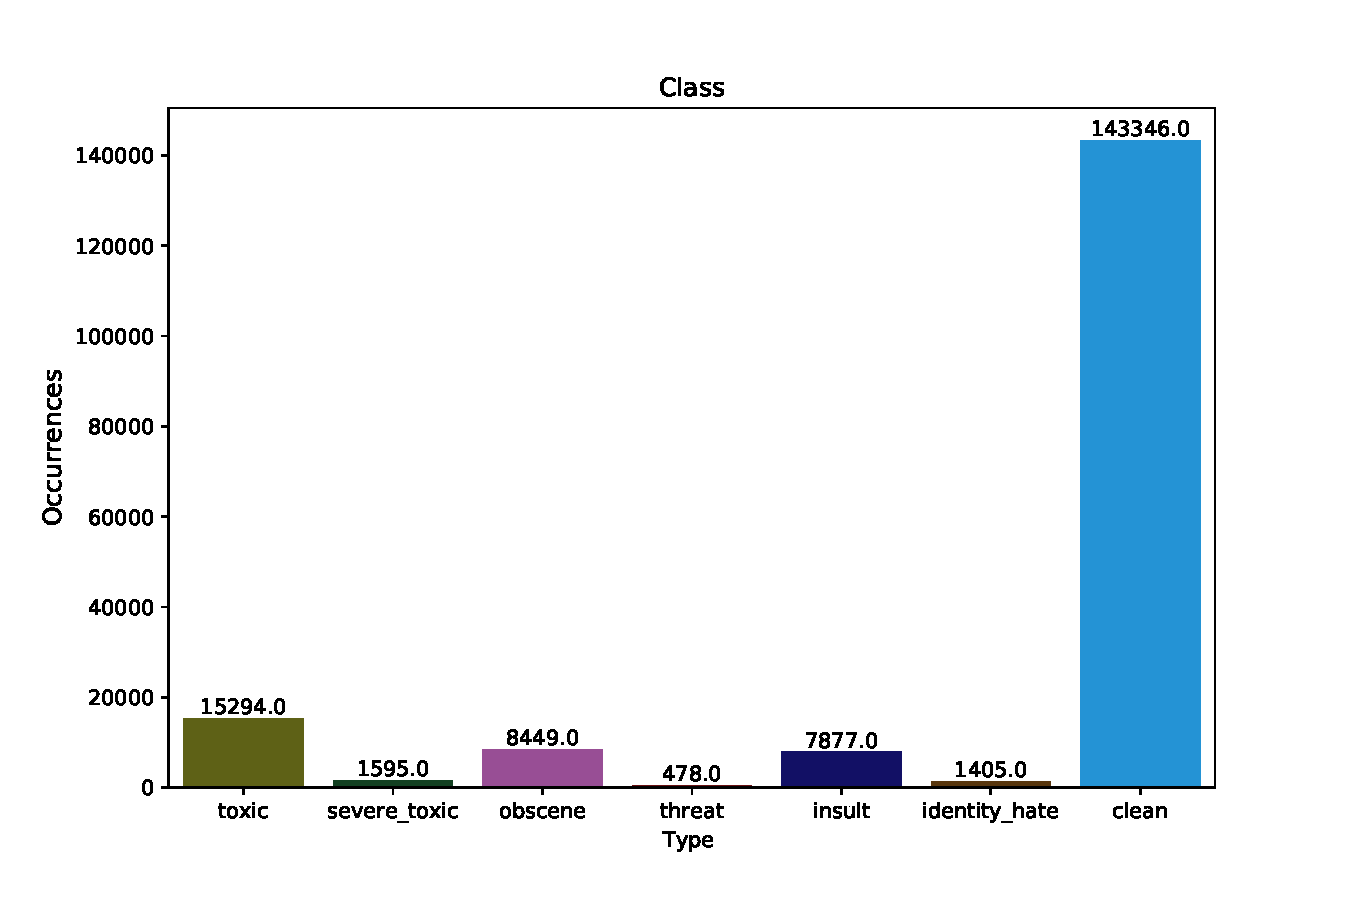
\includegraphics[scale=0.7]{figures/labels.pdf}
        \caption{Toxic comment dataset label distribution}
        \label{fig:labels}
    \end{figure}

    The plot shows that most of the comments are innocent and small number of comments are classified as any form toxic comment. The comments classified as severely toxic, threat and identity hate are rare compared to toxic, obscene and insult.
    
    An example of a comment is provided bellow with was labeled as both toxic and a threat.

    \begin{verbatim}
        ('Hi! I am back again!\nLast warning!\nStop undoing my edits or die!',
    \end{verbatim}

    As it can be seen, the comments are not clean and contain many signs, symbols and spelling errors that makes the classification problem based on word level vectors much harder.

    It's also helpful to look at word could of comments labeled with any of toxic comments labels (Figure \ref{fig:wordcloud}):

    \begin{figure}[!h]
        \centering
        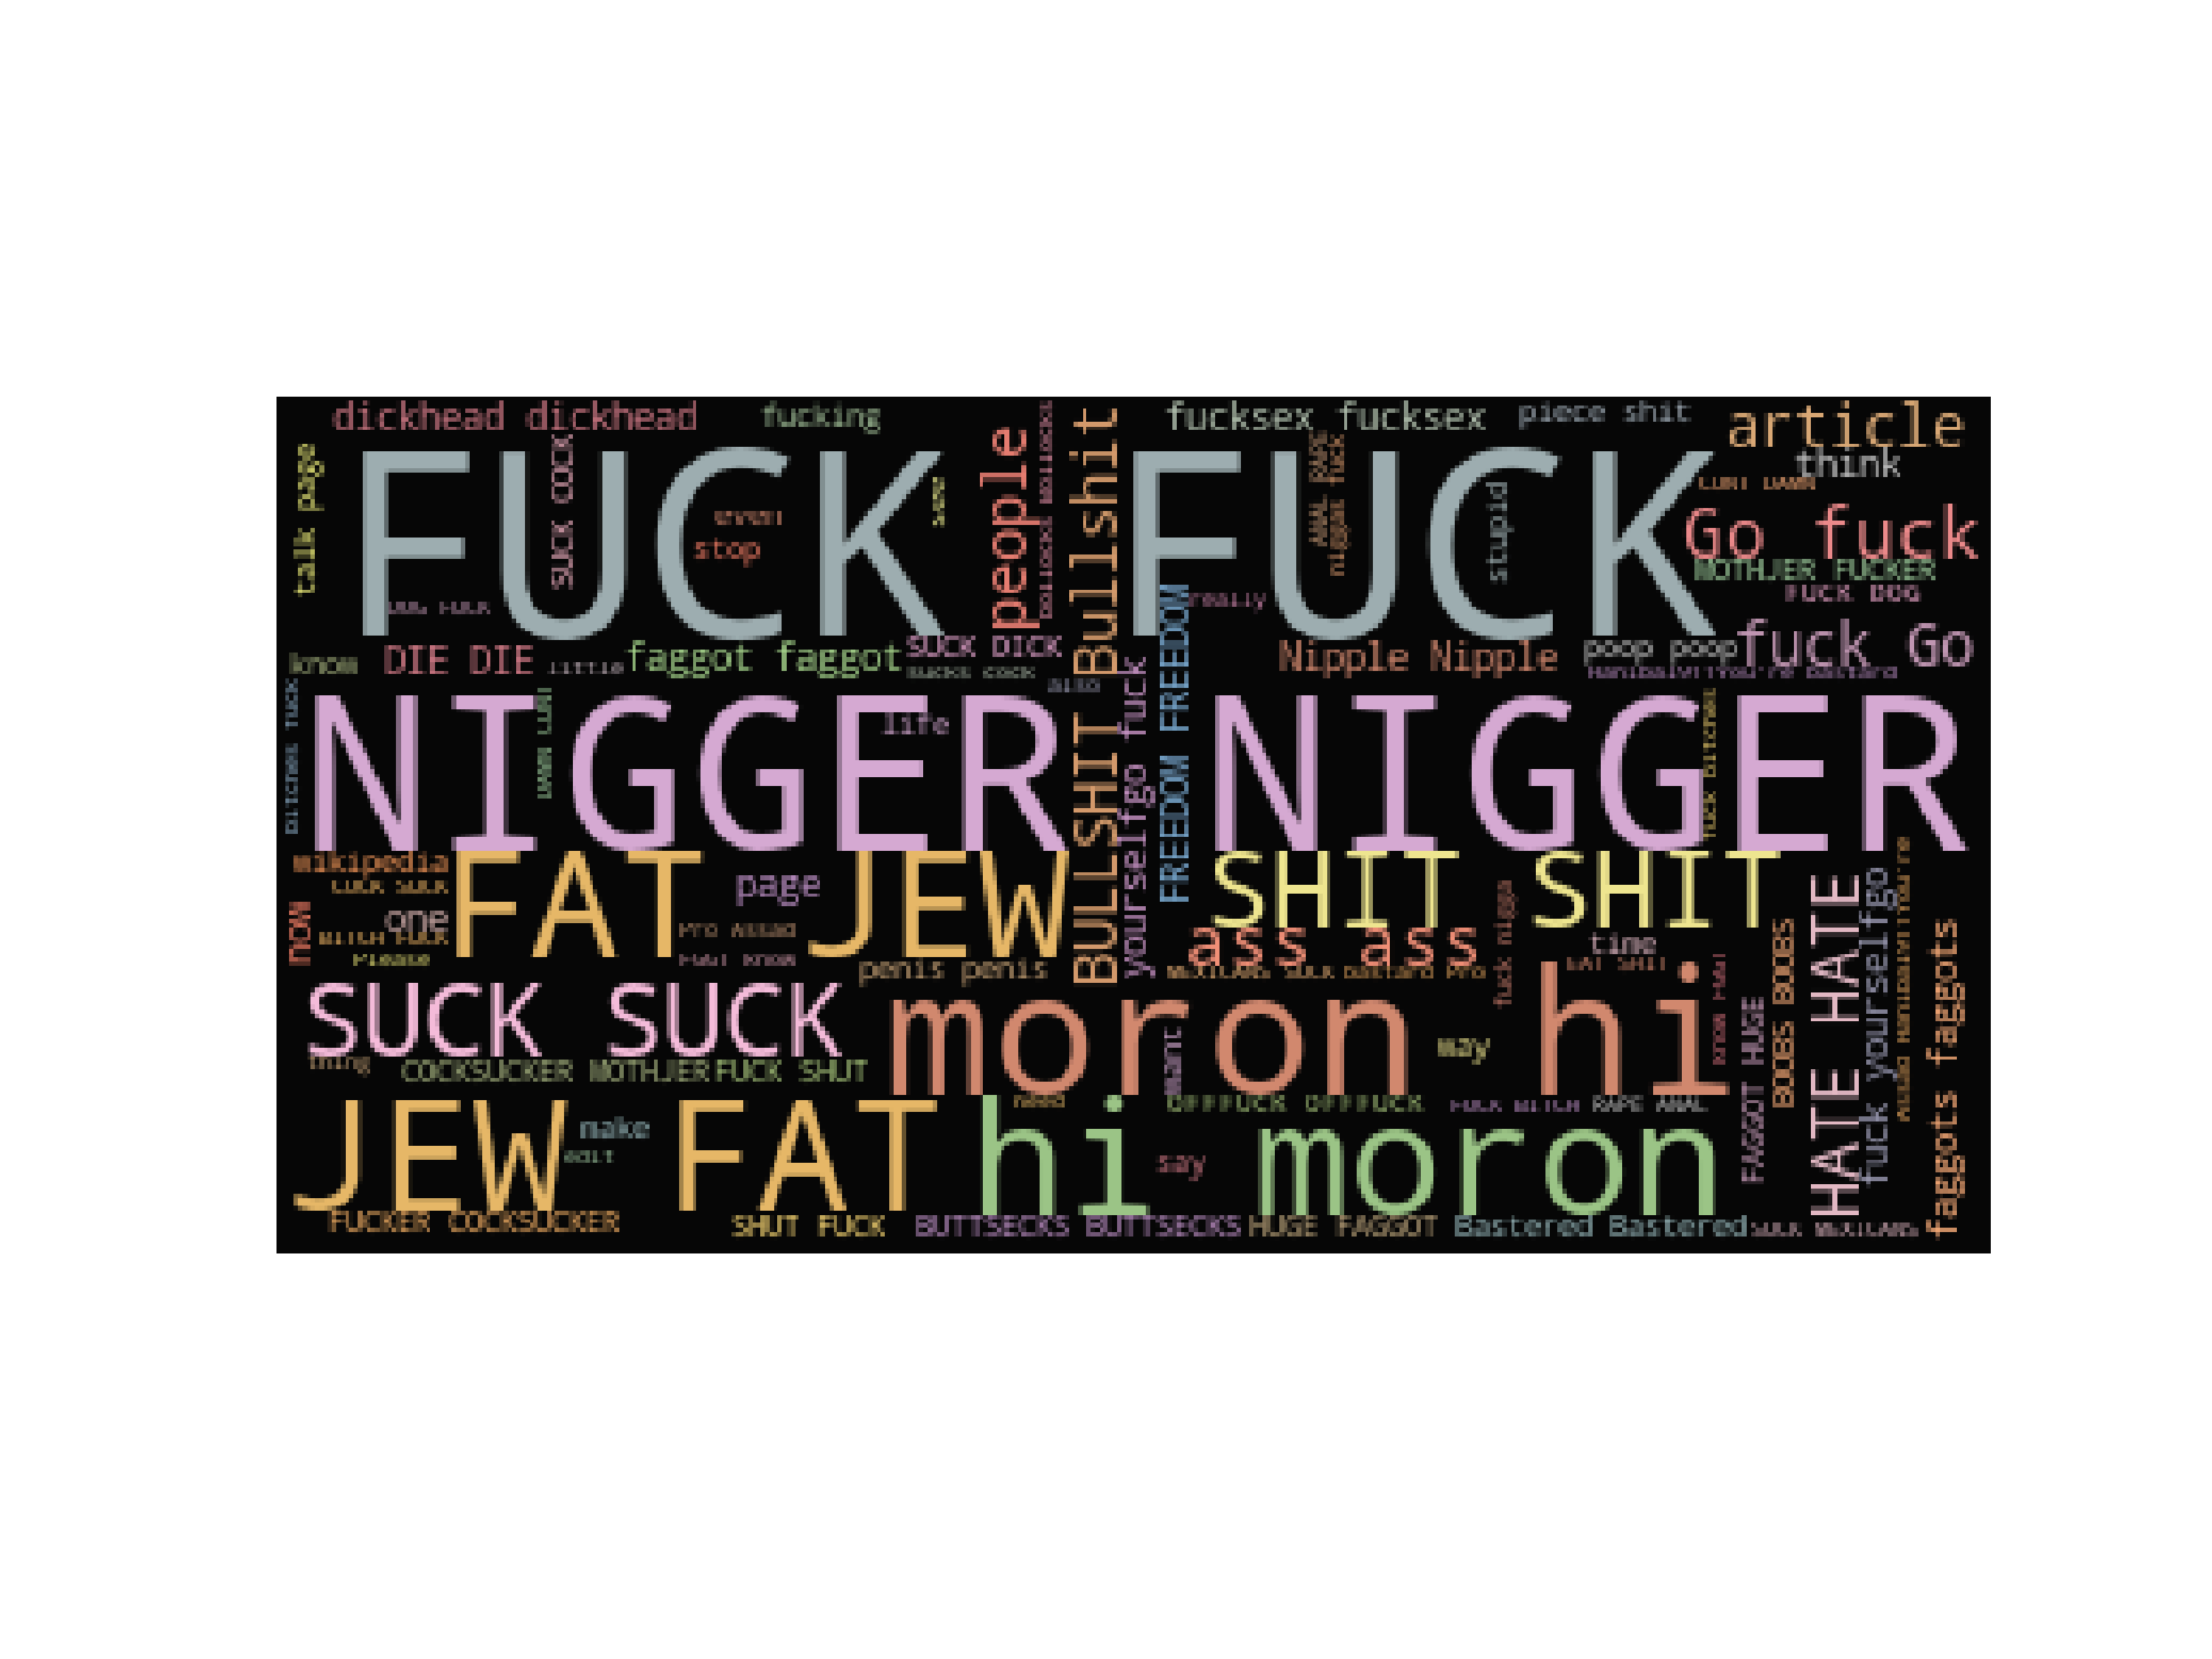
\includegraphics[scale=0.3]{figures/wordcloud.pdf}
        \caption{Toxic Comment WordCloud}
        \label{fig:wordcloud}
    \end{figure}


    The data will be divided in to 3:1:1 for training validation and testing. Since the labels are not balanced, during the training each batch of data will be sampled using a Stratified sampling method to expose the model to different class labels.

    \subsection{Algorithms and Techniques}

    Recurrent neural network architectures combining with attention mechanism,
    or neural attention model, have shown promising performance recently for
    the tasks including speech recognition, image caption generation,
    visual question answering and machine translation. 
    In the sequence labeling tasks,
    the model input is a sequence, and the output is the label of the
    input sequence. The major difficulty of sequence labeling is that when
    the input sequence is long, it can include many noisy or irrelevant parts.
    If the information in the whole sequence is treated equally, the noisy or
    irrelevant part may degrade the classification performance.
    The attention mechanism is helpful for sequence classification task because
    it is capable of highlighting important part among the entire sequence for
    the classification task.



    In this project, each comment is treated as set of features using pre-trained GloVe word embedding. A Bi-directional recurrent neural network with Gated Recurrent Units (GRU). Attention mechanism is added on top of the Bi-directional RNN which improve the performance of the model focusing on important parts of long sequence and reduce the effect of noise and unrelated information. The classification task is a multi-label classification where comments toxicity labels are not mutually exclusive.



    \subsection{Benchmark}

    The baseline chosen here in order to get better understanding of the problem from a general machine-learning perspective. To this end, the baseline model is chosen to be a logistic regression model based on Term Frequency-inverse document frequency data which can achieve column-wise log-loss of $0.05567$.



\section{Methodology}

    \subsection{Data Processing}

    The preprocessing is mostly done using functions available in data.py module. The preprocessing step  before training or testing consist of following steps:

    \begin{itemize}
        \item Preprocessing comments:
            \begin{itemize}
                \item tokenizing
                \item converting to lower-case letters
                \item removing stopwords
                \item normalizing numbers, date, ...
            \end{itemize}

        \item Vocabulary: creating dictionary of words with at least $count() > Thresh_hold$.
        \item Index to word: dictionary with keys equal to word index and values being a word in the vocabulary
        \item Word to index: dictionary with keys equal to vocabulary's word and value being words index.
        \item Sequence index file: a file containing sequence of word index for each comment.
    \end{itemize}

    During training, the pre-processed comment are read from sequence to index file and push to TensorFlow input placeholders. In addition, at the beginning of the training the word vectors corresponding to the words in the vocabulary are extracted from pre-trained GloVE word vector with $6$ Billion words and specified word vector dimension.

    The preprocessing process has the following adjustable parameters:

    \begin{itemize}
        \item Word frequency threshold
        \item GLoVe word vector dimension (50, 100, 200)
        \item Using trainable or not trainable word vector tensor
        \item Maximum input sequence length
    \end{itemize}



    \subsection{Implementation}

    \subsubsection{Text Classification with Recurrent Neural Networks}

    The architecure used in this work is Recurrent Neural Network (RRN) that takes the sequence of words index and an encode the information in the text in the last output layer. The last output layer of the RNN is passed through two feed forward layers and a final $1 \times 6$ layer where a element wise sigmoid function is applied and a multi-label predictions are generated. Since some of the comments are quite long, a Bi-directional RNN is used which has two Gated Recurrent Cells (GRU) for forward and backward processing of the input sequence and outputs the concatenated output oof the forward and backward cell [figure \ref{figure:bi-rnn}].
    
    \begin{figure}
        \centering
        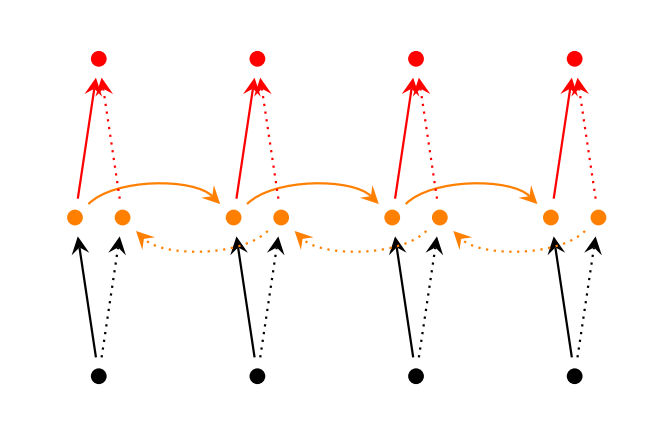
\includegraphics[scale=0.6]{bi_rnn.png}
        \caption{Bi-directional RNNS}
        \label{figure:bi-rnn}
    \end{figure}
    

    \subsection{Refinement}

    \subsubsection{Attention Mechanism}
    Since not all words contribute equally to the representation of the sequence meaning we need to use an attention mechanism [\cite{yang2016hierarchical}] that extract important words to the meaning of the sequence and aggregates the presentation of informative words to form a sentence vector from [figure \ref{fig:attention}
    
    \begin{align}
        u_{it} = tanh(W_w h_{it} + b_w) \\
        \alpha_{it} = \frac{exp(u_{it}^T u_w)}{\sum_t exp(u_{it}^T u_w)} \\
        o = \sum_t \alpha_{it}h_{it} 
    \end{align}
    
    where the word annotation $h_{it}$ is passed to a one-layer MLP to get $u_it$ as hidden representation $h_it$  the importance of the word is measured by comparing $u_{it}$ to a word context vector $u_w$ and then passed through a softmax function to get normalized importance weight $\alpha_{it}$ and the output vector is weighted sum of word annotation based of the weights. The context vector is randomly initialized and jointly learned during the training process.

    \begin{figure}
        \centering
        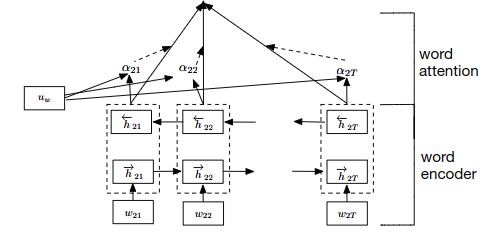
\includegraphics[scale=0.7]{attention.png}
        \caption{Attention Mechanism \cite{yang2016hierarchical}}
        \label{fig:attention}
    \end{figure}

    The completed TensorFlow computational graph can be seen in Figure [\ref{fig:tensorflow}]

    \begin{figure}
        \centering
        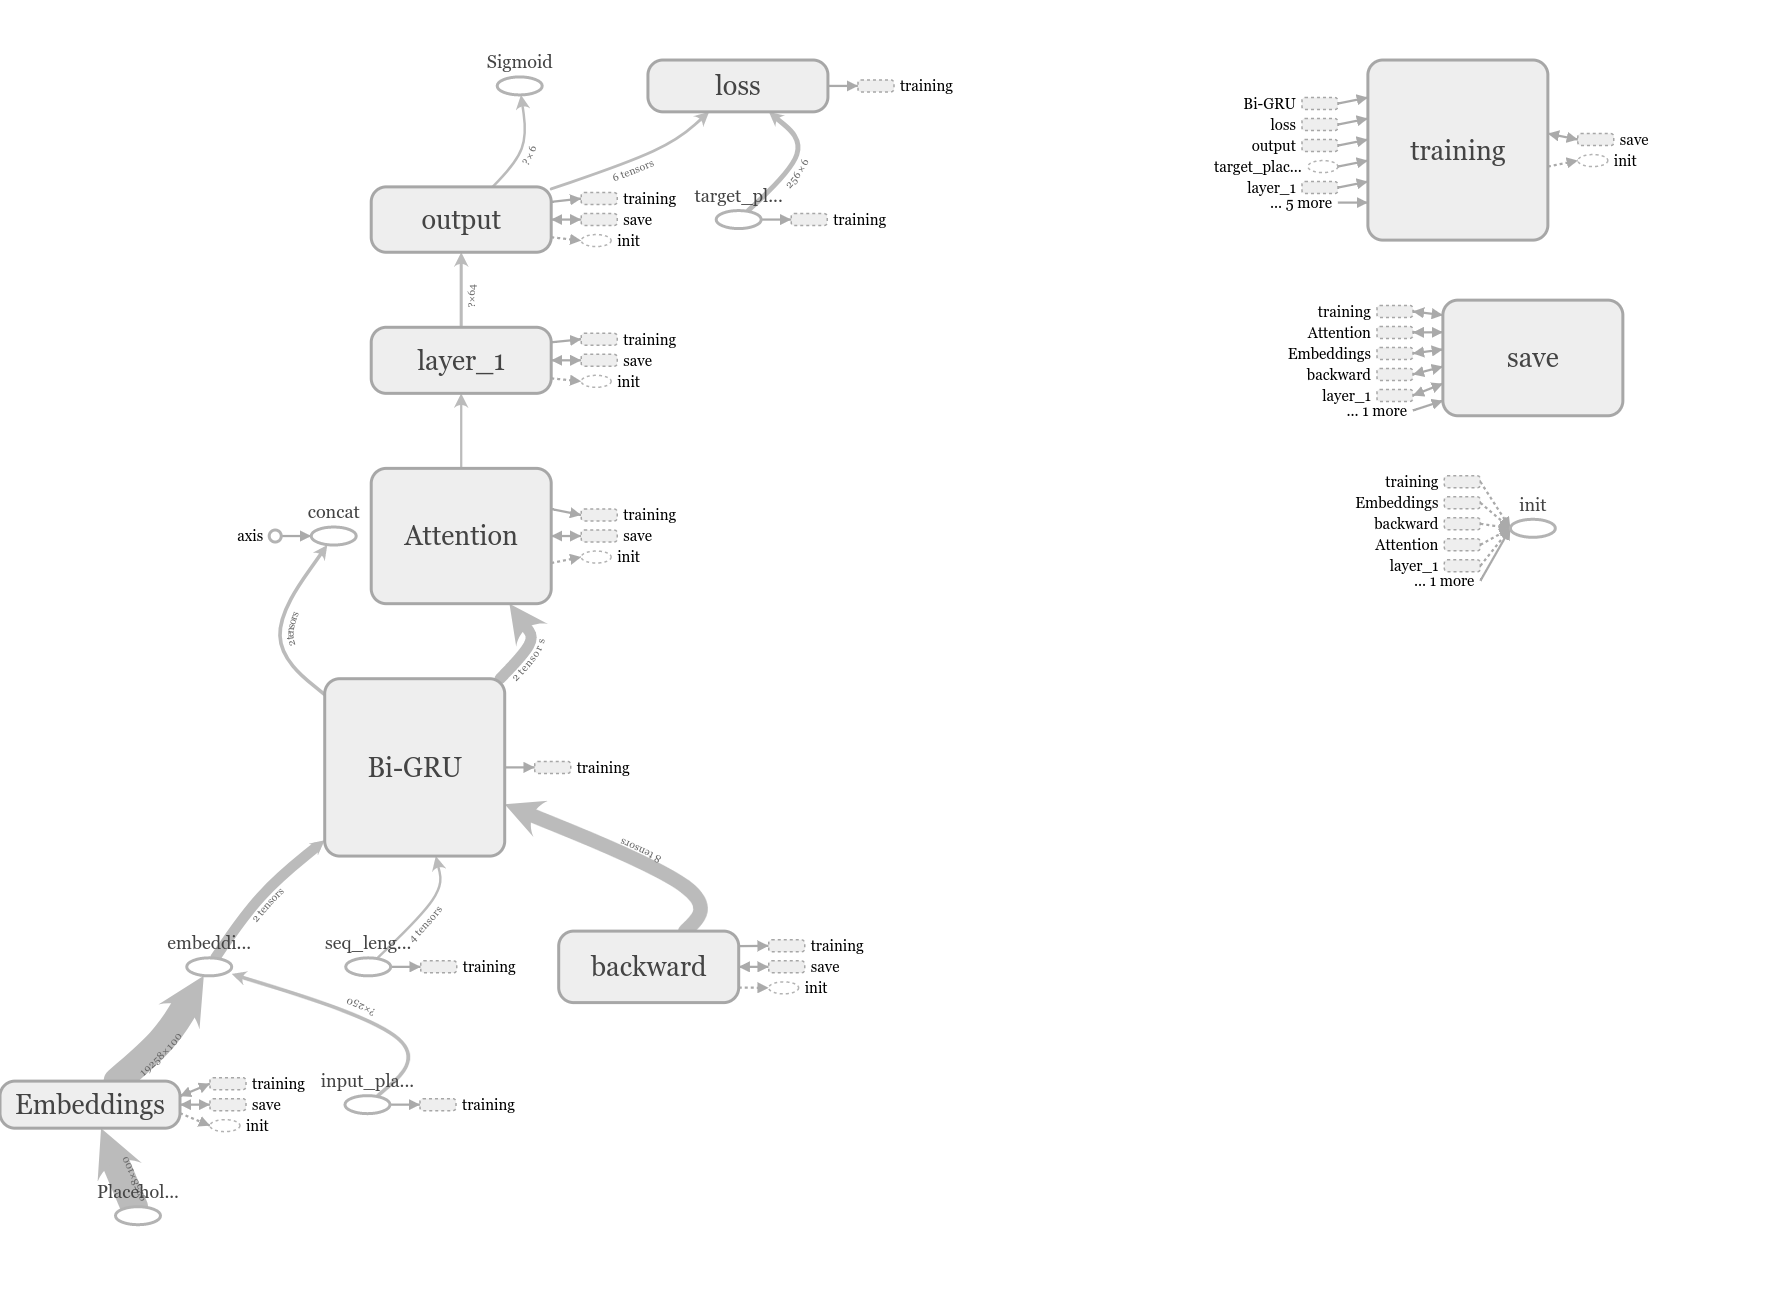
\includegraphics[scale=0.3]{tensorflow.png}
        \caption{TensorFlow computational graph for sequence classification model with attention mechanism}
        \label{fig:tensorflow}
    \end{figure}

    \subsubsection{Other Measures}

    In addition to the attention layer other measures such as dropout layers, exponential learning rate decay were used to reduce the log-loss and improve the model generalization. 


\section{Results}

    \subsection{Model Evaluation and Validation}

    During development process, the training data was split into training ($90\%$) and validation ($10\%$) sets. Since this project is part of Kaggle competition, instead of using a test set the submission result is used as a metric for final evaluation of the model.

    The final description of the final model is as follows:


    \begin{itemize}
        \item Batch Size = 256
        \item Embedding dimension = 100
        \item Number of GRU Cells = 128
        \item Feed-forward layers = 128
        \item Attention size = 256
        \item Maximum input sequence length = 250
    \end{itemize}

    An early-stopping mechanism is implemented to automatically save model weights corresponding to best evaluation log-loss and stop the training to prevent over-fitting to the training set.


    \subsection{Justification}

\section{Conclusion}


    \subsection{Free-Form Visualization}


    \subsection{Reflection}

    \subsection{Improvement}




\bibliographystyle{plainnat}
\bibliography{bibliography.bib}
    
\end{document}